\section{Data Acquisition and Signal-Processing Diagnostics}
\label{app:data-diagnostics}

This appendix presents additional diagnostic evidence supporting the
data-quality screening, operational-state detection and physics-informed
signal-processing decisions described in Sections \ref{sec:data-understanding} and \ref{sec:data-preparation}.

\begin{figure}[p]
    \centering
    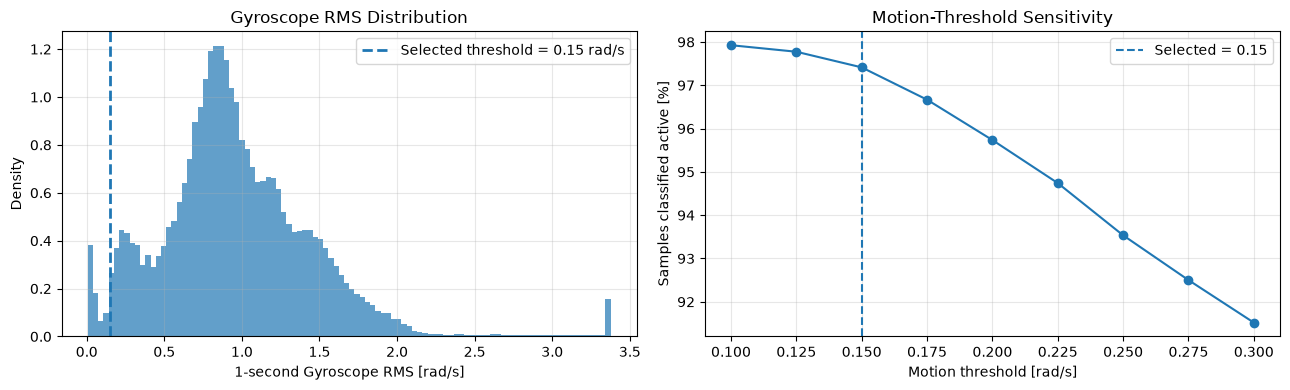
\includegraphics[width=\textwidth]
    {figures/motion-threshold-selection.png}
    \caption{Diagnostic analysis used to select the gyroscope-based motion
    threshold. The left panel shows the distribution of the one-second
    gyroscope RMS envelope and the selected threshold of 0.15~rad/s.
    The right panel shows the sensitivity of the proportion of samples
    classified as active to alternative threshold values.}
    \label{fig:appendix-motion-threshold}
\end{figure}



\begin{figure}[p]
    \centering
    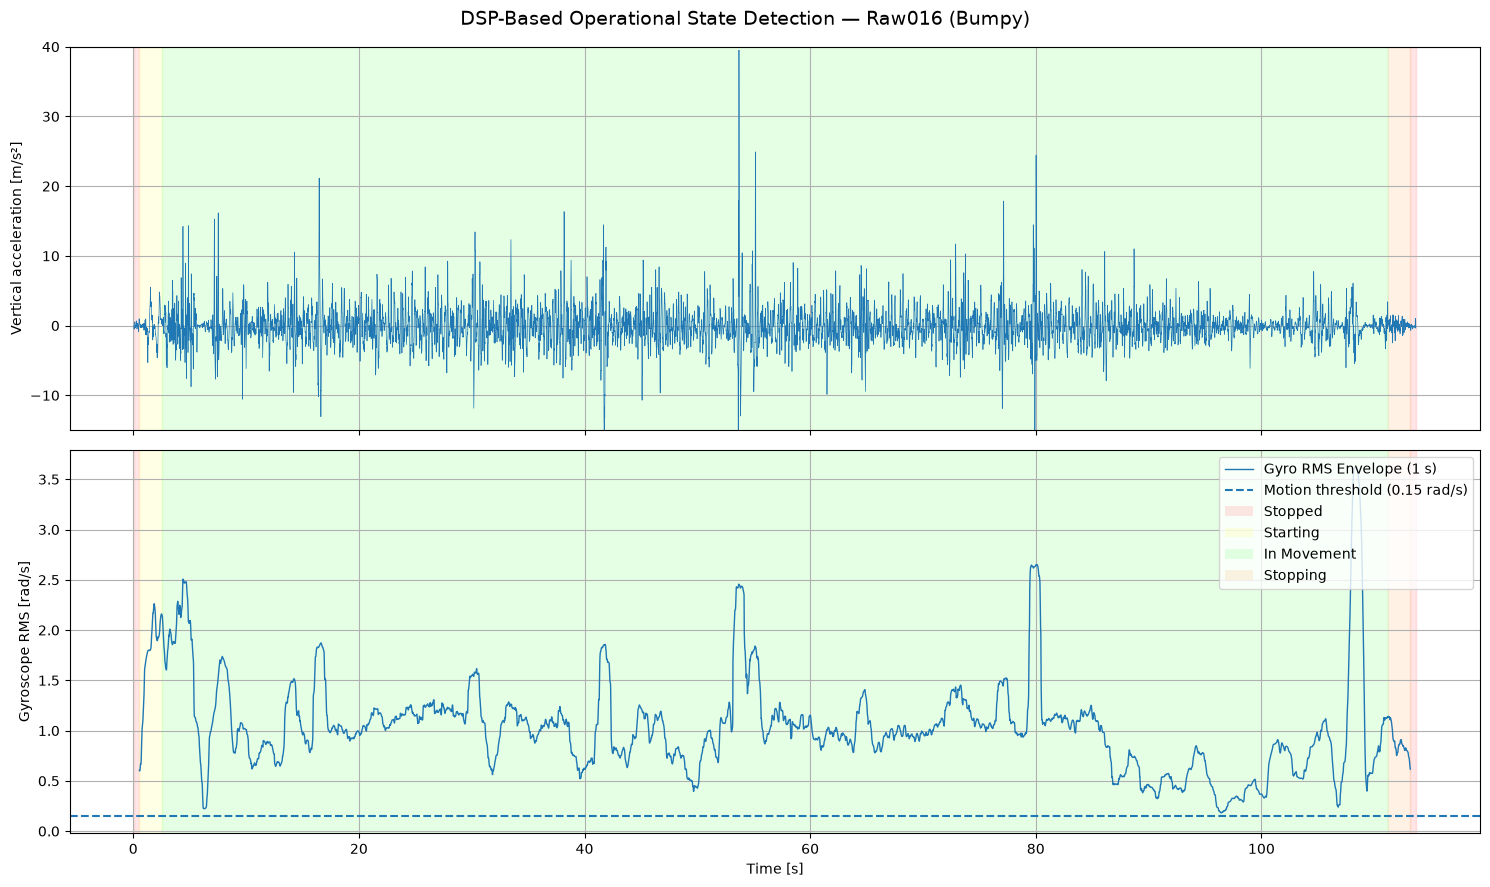
\includegraphics[width=\textwidth]
    {figures/dsp-based-state-detection-example.png}
    \caption{Example of DSP-based operational-state detection for a Bumpy
    recording. The upper panel shows vertical dynamic acceleration and the
    lower panel the smoothed gyroscope RMS envelope. Background shading marks
    samples classified as Stopped, Starting, In Movement and Stopping. Only
    stable In Movement regions were retained for feature extraction.}
    \label{fig:appendix-state-detection}
\end{figure}

\clearpage